%\documentclass[article,amsmath,amssymb,reprint,onecolumn]{revtex4-1}
\documentclass[aip,amsmath,amssymb,reprint,onecolumn]{revtex4-1}
\usepackage{graphicx} % Include figure files
\usepackage{dcolumn} % Align table columns on decimal point
\usepackage{bm} % bold math
\usepackage{color,xcolor}
\usepackage{amsfonts,amsmath,amssymb}
\usepackage{titlesec}
\usepackage{helvet}
\usepackage{hyperref}

\newcommand{\citemark}{\color{red}}

\renewcommand\thesection{\arabic{section}}
\renewcommand\thesubsection{\arabic{subsection}}
\renewcommand\thesubsubsection{\arabic{subsubsection}}
\renewcommand{\familydefault}{\sfdefault} % sf font for the whole text

\newcommand\putright[2]{ % #1 = number of lines to lower the figure, #2 = content
    \leavevmode\vadjust{\hfill\smash{\lower\dimexpr#1\baselineskip-2.5\lineskip\relax\llap{#2}}}\ignorespaces
}

\setcounter{tocdepth}{5}
\setcounter{secnumdepth}{5}

\definecolor{darkcyan}{rgb}{0.0, 0.50, 0.55}
\definecolor{navyblue}{rgb}{0.0, 0.0, 0.5}
\definecolor{lightgray}{rgb}{0.7, 0.7, 0.7}
\titleformat{\section}  {\normalfont\sffamily\Large\bfseries\color{cyan}} {\thesection}{1em}{}
\titleformat{\subsection}  {\normalfont\sffamily\large\bfseries\color{darkcyan}} {\thesection.\thesubsection}{1em}{}
\titleformat{\subsubsection}  {\normalfont\sffamily\it\bfseries\color{black}} {\thesection.\thesubsection.\thesubsubsection}{1em}{}


\begin{document}

\putright{3}{

\includegraphics[height=.05\textwidth]{hkust.png}
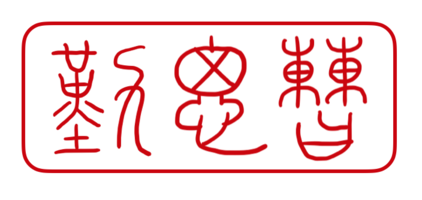
\includegraphics[height=.05\textwidth]{logo.png}
}

\title{\huge 3DRISMHI User Manual}% Force line breaks with \\

\maketitle

{\large Version 0.246}

\tableofcontents

\setlength{\parskip}{0.4\baselineskip}%

\section{Overview}

The 3DRISMHI is an open-source software package to calculate the atomic distributions of solvents around given solutes based on integration equation theory (IET) or liquid and hydrophobicity induced density inhomogeneity (HI) theory \cite{Cao_Xuhu_JCP_2015, Cao_Xuhu_MP_2018, Cao_Huang_AdTS_2019}. Based on the structure of solutes, the force field parameters of solute, the solvent-solvent correlations (provided in the package or generated from MD simulations), the molecular structure of solvents (provided in the package or generated from structures) and some experimental parameters (provided in the package or modify youself), the 3DRISMHI can efficiently calculate the solvent density distrubution.

The 3DRISMHI can use multi cores (of one computer) to speed up the calculation. The memory required to perform a 3DRISMHI calculation is probably huge, so by default the allocated memory will not exceed the physical RAM installed on your computer (you can bypass this check via -ignore-memory-capacity). 3DRISMHI doesn't provide MPI or GPU paralleling due to highly and frequently exchange of memories.

The 3DRISMHI is an independent software that can run on Linux, Mac OS, Windows Subsystem Linux and Windows Cygwin. The only required package is FFTW version 3. More features will be avaiable if compiled with the following packages: libz, GROMACS. The 3DRISMHI doesn't have any graphical interface, and need to run in terminals or computer clusters.

The 3DRISMHI is developed and maintained by Siqin Cao (PhD) from the Hong Kong University of Science and Technology, and supported by Xuhui Huang (Professor PhD).

%\noindent\makebox[\linewidth]{\rule{\linewidth}{0.4pt}}

\section{Theory}

\subsection{Force field}

The 3DRISMHI adopts the well received atomic potential model to compute the solute-solvent interactions, which consists of a Lennard-Jones (LJ) potential and an electrostatic potential (Coulomb by default):
\begin{equation*}
    v_{ij}(r_{ij}) = 4\varepsilon_{ij}\left(\left(\frac{\sigma_{ij}}{r_{ij}}\right)^{12} - \left(\frac{\sigma_{ij}}{r_{ij}}\right)^6 \right) + \frac{q_iq_j}{4\pi\varepsilon_0r_{ij}}
\end{equation*}

In the LJ potential, the mixing rule of $\varepsilon$ is
\begin{equation*}
    \varepsilon_{ij}=\sqrt{\varepsilon_i\varepsilon_j}
\end{equation*}
Two mixing rules of $\varepsilon$ are provided:
\begin{equation*}\begin{split}
    &{\rm arithmetic:\ } \sigma_{ij} = \frac{\sigma_i+\sigma_j}{2} \\
    &{\rm geometric:\ \ } \sigma_{ij} = \sqrt{\sigma_i\sigma_j} \\
\end{split}\end{equation*}

Several electrostatic potentials are provided:
\begin{equation*}\begin{split}
    &{\rm dielectric:} v^{\rm ES}_{ij}(r_{ij}) = \frac{q_iq_j}{4\pi\varepsilon_0\varepsilon_rr_{ij}} \\
    &{\rm Yukawa:\ \ \ \ } v_{ij}(r^{\rm ES}_{ij}) = \frac{q_iq_j}{4\pi\varepsilon_0}\frac{e^{-\kappa r_{ij}}}{r_{ij}} \\
\end{split}\end{equation*}
where $\varepsilon_r$ is the dielectric constant, and $\kappa=1/r_{\rm Yukawa}$ is the Debey wavenumber (or overridden by a user defined number).

The Particle Mesh Ewald (PME) method is adopted to calculate the Coulomb potential:
\begin{equation*}\begin{split}
    \frac{1}{r} = \frac{{\rm erf}(\gamma r)}{r} + \frac{{\rm erfc}(\gamma r)}{r}
\end{split}\end{equation*}
where $\gamma=2/r_C$, and $r_C$ is the cutoff distance for short range part of Coulomb interactions. The long range part of the Coulomb potential ${\rm erfc}(\gamma r)/r$ and the Yukawa potential are both calculated with Fourier transformations.

\subsection{Equation one of IET: the Ornstein-Zernike equation}

The OZ equation:
\begin{equation}\begin{split}\label{eq:OZ}
    h_{ij}(\vec{r}_i,\vec{r}_j) &= c_{ij}(\vec{r}_i,\vec{r}_j) + \int c_{ik}(\vec{r}_i,\vec{r}_k)h_{kj}(\vec{r}_k,\vec{r}_j) \rho^b_kd^3\vec{r}_k \\
    &\equiv c_{ij}(\vec{r}_i,\vec{r}_j) + c_{ik}(\vec{r}_i,\vec{r}_k) *_k h_{kj}(\vec{r}_k,\vec{r}_j)
\end{split}\end{equation}

The 3DSSOZ or 3DRISM equation:
\begin{equation}\label{eq:SSOZ}
    h_{ij} = c_{ij} + c_{ik} *_k \hbar_{kj}
\end{equation}

In SSOZ, the total solvent-solvent correlation function consists of the inter-molecular correlation $h_{kj}$ and the intra-molecular correlation\cite{Cao_Huang_AdTS_2019} $\delta_{kj}(r_{kj}-b_{kj})$ :
\begin{equation}\label{eq:hbar}
    \hbar_{kj} = h^{\rm inter}_{kj} + h^{\rm intra}_{kj} = h_{kj} + \delta_{kj}(r_{kj}-b_{kj})
\end{equation}
Generally in the RISM field, this is written as \cite{Ratkova_Maxi_CR_2015}:
\begin{equation}\label{eq:omega-correlatin}
    1 + \hbar_{kj} = 1 + h^{\rm inter}_{kj} + h^{\rm inner}_{kj} = \omega_{kj} + h_{kj} = \chi_{kj}
\end{equation}

The 3DRISM equation with the renormalization of Coulomb:
\begin{equation}\begin{split}\label{eq:3DRISM}
    &h_{ij} = c_{ij}^{\rm R} + c_{ik}^{\rm LR} *_k \hbar_{kj} + h_{ij}^{\rm LR} \\
    &h_{ij}^{\rm LR} = c_{ij}^{\rm LR} + c_{ik}^{\rm LR} *_k \hbar_{kj} \\
    &c_{ij}^{\rm LR} = - v_{ij}^{\rm LR}
\end{split}\end{equation}

\subsection{Equation two of IET: the closure equation}\label{sec:closure}

The density functional form of the closure equation is:
\begin{equation}\label{eq:closure-original}
    g_{ij} = \exp\left[ -v_{ij} + \int c_{ik}*_k\frac{\partial\hbar_{kj}(\lambda)}{\partial\lambda} d\lambda \right]
\end{equation}
By expanding the integration, the general form of the closure equation can be derived:
\begin{equation}\label{eq:closure}
    g_{ij} = \exp\left[ -v_{ij} + \int c_{ik}*_k\hbar_{kj} + B_{ij} \right] = \exp\left[ -v_{ij} + h_{ij} - c_{ij} + B_{ij} \right]
\end{equation}
where $B_{ij}$ is called the bridge function.

This software support the following closures \cite{Ratkova_Maxi_CR_2015, Cao_Huang_AdTS_2019}, and choose the closure(s) that best suitable for your solvent molecule(s):

\subsubsection{HNC/MSA based closures}

The Hyper-Netted-Chain (HNC) closure:
\begin{equation}\label{eq:HNC}
    g_{ij} = \exp\left[ -v_{ij} + h_{ij} - c_{ij} \right]
\end{equation}

The Mean-Spherical-Approximation (MSA):
\begin{equation}\begin{split}\label{eq:MSA}
    &v_{ij}<\infty: c_{ij} = -v_{ij} \\
    &v_{ij}\rightarrow\infty: h_{ij} = -1
\end{split}\end{equation}

The Kobryn-Gusarov-Kovalenko (KGK) closure:
\begin{equation}\begin{split}\label{eq:KGK}
    g_{ij} = \max\left\{ 0, 1-v_{ij}+h_{ij}-c_{ij} \right\}
\end{split}\end{equation}

The Partial-Linear-HNC (PLHNC) closure:
\begin{equation}\begin{split}\label{eq:PLHNC}
    g_{ij} = \begin{cases}
        \exp\left[-v_{ij}+h_{ij}-c_{ij}\right], &\ln g_{ij}\le C\\
        -v_{ij}+h_{ij}-c_{ij} - C + e^C, &\ln g_{ij}\ge C
    \end{cases}
\end{split}\end{equation}

The Kovalenko-Hirata (KH) closure:
\begin{equation}\begin{split}\label{eq:KH}
    g_{ij} = \begin{cases}
        \exp\left[-v_{ij}+h_{ij}-c_{ij}\right], &g_{ij}\le 1\\
        1-v_{ij}+h_{ij}-c_{ij}, &g_{ij}\ge 1
    \end{cases}
\end{split}\end{equation}

The PSE-n expansion of the HNC closure:
\begin{equation}\begin{split}\label{eq:PSEn}
    g_{ij} = \begin{cases}
        \exp\left[-v_{ij}+h_{ij}-c_{ij}\right], &g_{ij}\le 1\\
        1+\sum_{m=1}^n\frac{1}{n!}(-v_{ij}+h_{ij}-c_{ij})^n, &g_{ij}\ge 1
    \end{cases}
\end{split}\end{equation}
(PSE1 is equivalent to KH. This software support PSE1 to PSE10)

\subsubsection{Bridge function based closures}

The Percus-Yevick (PY) closure:
\begin{equation}\begin{split}\label{eq:PY}
    g_{ij} = e^{-v_{ij}}\left(1 + h_{ij}-c_{ij}\right)
\end{split}\end{equation}

The HNC-Bridge (HNCB) closure:
\begin{equation}\label{eq:HNCB}
    g_{ij} = \exp\left[ -v_{ij} + h_{ij} - c_{ij} - \frac{1}{2}\left(h_{ik}*_k\hbar_{kj}\right)^2\right]
\end{equation}

The D2 (D2 with {\bf -cmd ssoz}) closure \cite{Cao_Xuhu_JCP_2015, Cao_Huang_AdTS_2019}:
\begin{equation}\label{eq:HNCB}
    g_{ij} = \exp\left[ -v_{ij} + h_{ij} - c_{ij} - \frac{1}{2}\left(c_{ik}*_k\hbar_{kj}\right)^2\right]
\end{equation}

The D2-MSA (D2 with {\bf -cmd rism}) closure \cite{Cao_Xuhu_MP_2018, Cao_Huang_AdTS_2019}:
\begin{equation}\label{eq:D2MSA}
    g_{ij} = \exp\left[ -v^{\rm SR}_{ij} + h_{ij} - c^{\rm R}_{ij} - \frac{(h_{ij} - c^{\rm R}_{ij})^2}{2}\right]
\end{equation}

The Martynov-Sarkisov (MS) closure:
\begin{equation}\label{eq:MS}
    g_{ij} = \exp\left[ -v_{ij} + \sqrt{1 + 2(h_{ij} - c_{ij})} - 1\right]
\end{equation}
In order to avoid the numerical crash at $h_{ij} - c_{ij}<-0.5$, the MSHNC (MSHNC) closure is also implemented in 3DRISMHI:
\begin{equation}\begin{split}\label{eq:MSHNC}
    g_{ij} = \begin{cases}
        \exp\left[-v_{ij}+h_{ij}-c_{ij}\right], &h_{ij}-c_{ij}\ge 0\\
        \exp\left[ -v_{ij} + \sqrt{1 + 2(h_{ij} - c_{ij})} - 1\right], &h_{ij}-c_{ij}\le 0
    \end{cases}
\end{split}\end{equation}

The BPGG closure:
\begin{equation}\label{eq:BPGG}
    g_{ij} = \exp\left[ -v_{ij} + \left(1 + \alpha(h_{ij} - c_{ij})\right)^{1/\alpha} - 1\right]
\end{equation}
In order to avoid the numerical crash at $h_{ij} - c_{ij}<-1/\alpha$, the BPGGHNC (BPGGHNC) closure is implemented in 3DRISMHI:
\begin{equation}\begin{split}\label{eq:BPGGHNC}
    g_{ij} = \begin{cases}
        \exp\left[-v_{ij}+h_{ij}-c_{ij}\right], &h_{ij}-c_{ij}\ge 0\\
        \exp\left[ -v_{ij} + \left(1 + \alpha(h_{ij} - c_{ij})\right)^{1/\alpha} - 1\right], &h_{ij}-c_{ij}\le 0
    \end{cases}
\end{split}\end{equation}

The Modified Verlet bridge (VM):
\begin{equation}\begin{split}\label{eq:VM-and-MHNC}
    g_{ij} = \exp\left[-v_{ij} + h_{ij} - c_{ij} - \frac{1}{2}\frac{(h_{ij}-c_{ij})^2}{1 + \alpha\times(h_{ij}-c_{ij})}\right]
\end{split}\end{equation}
where $\alpha$ is a constant. In particular, the modified HNC (MHNC) closure takes $\alpha=0.8$.

The MP closure:
\begin{equation}\label{eq:MP}
    g_{ij} = e^{-v_{ij}}\left[ (1+\alpha)e^{(h_{ij}-c_{ij})/(1+\alpha)} - \alpha \right]
\end{equation}

\subsubsection{User defined closures}

{\it

This software also provids three user defined closures: ``user1'', ``user2'' and ``user3''. The name of these three closures can be changed in line 197-199 of \texttt{rismhi3d.cpp}, and the code to perform these closures are in line 230-244 of \texttt{main-rism.cpp}. The default code of these closures are doing HNC closure, and please change them with your own code if you want to add more closure equations.

The closures like HNCB requires additional convolutions of $h_{ik}*_k\hbar_{kj}$. This kind of additional convolution is performed in the function prepare\_closure() of \texttt{main-rism.cpp}. Please follow the code of HNCB to include additional terms in your new closures.

}

\subsection{Equation three of 3DRISMHI: the HI equation}

In the hydrophobicity induced density inhomogeneity (HI) theory, the global average density constants $\rho^b_\gamma$ is substituted with spacial inhomogeneous local average densities $\rho^S_\gamma(\vec{r}_\gamma) = \rho^b_\gamma n_\gamma(\vec{r}_\gamma)$. This density is slowly varying and is called the slowly varying component of the liquid density in the LCW theory, or the dimensionless density in the HI theory. The dimensionless density is calculated with the HI equation:
\begin{equation}
    \ln n_\gamma - \ln\lambda = \zeta_{\gamma\mu}*_\mu n_\mu\Theta(\rho_\mu-0^+) + ABe^{(1-1/n_\gamma)/A}
\end{equation}

The final density distribution of liquid in the HI theory is:
\begin{equation}
    \rho_\gamma(\vec{r}_\gamma) = \rho^b_\gamma n_\gamma(\vec{r}_\gamma) g_\gamma(\vec{r}_\gamma)
\end{equation}

\subsection{Self-consistent field iterations}

Both the RISM equation and the HI equation are solved in a self-consistent-field (SCF) manner. The SCF iterations of HI is simply done in the following way:
\begin{equation}
    \ln n_\gamma^{(n+1)} = \ln\lambda + \zeta_{\lambda\mu}*_\mu n_\mu^{(n+1)}\Theta(\rho_\mu-0^+) + ABe^{(1-1/n_\gamma^{(n+1)})/A}
\end{equation}
while the SCF iterations of RISM is performed as follows:
\begin{equation}\begin{split}
    &g^{(n+1)} = \exp\{-v + c^{(n)}*\hbar + B^{(n)}\} \\
    &c^{(n+1)} = g^{(n+1)} - 1 - c^{(n)}*\hbar
\end{split}\end{equation}

In both SCF iterations of RISM and HI, the Direct Inversion in the Iterative Subspace (DIIS) method \cite{Luchko_JCTC_2010,Gusarov_JCC_2012,Peter_CPL_1980} can be used to celerate and stabilize the convergence of SCF iterations. For a self-consistent equation $\textbf{f} = g(\textbf{f})$, the DIIS method adopts a linear combination of the approximation errors from the previous iterations to predict the next step,
\begin{equation}\begin{split}\label{eq.DIIS}
    \textbf{f}_{n+1} = \textbf{f}_{n} + \sum_i (\textbf{f}_i - g(\textbf{f}_i))c_i
\end{split}\end{equation}
where the coefficients $c_i$ are calculated from the minimization of the historical error,
\begin{equation}\begin{split}\label{eq.DIIS-Larange}
    L = \sum_i\Big|\textbf{f}_i - g(\textbf{f}_i)\Big|^2 + \lambda\left(\sum_ic_i - 1\right)
\end{split}\end{equation}

%\noindent\makebox[\linewidth]{\rule{\linewidth}{0.4pt}}

\section{Compilation guidance}

\subsection{Tools of the package}

There are four major tools in the 3DRISMHI package that needs to be installed:

\begin{itemize}
    \item \texttt{rismhi3d} : perform RISM/HI calculation
    \item \texttt{ts4sdump} : decode the binary (or compressed) data of grid-based distributions that generated by \texttt{rismhi3d}
    \item \texttt{gmxtop2solute} : the tool to generate the solute forcefield file from the TOP file of GROMACS. The compilation of \texttt{gmxtop2solute} does not require GROMACS.
    \item \texttt{gensolvent} : the tool that helps to generate the solvent setting file
\end{itemize}

\subsection{System requirement}

System requirement:

\begin{itemize}
    \item One of the following operation systems:
    \begin{itemize}
        \item Linux 4 and above (4.15 recommended)
        \item Mac OS 10.6 and above (10.14 recommended)
        \item Windows Cygwin
        \item Windows Subsystem Linux
    \end{itemize}
    \item C++03 and above (C++11 recommended)
\end{itemize}

Library requirement:

\begin{itemize}
    \item {\bf FFTW3 with double precision} (required)
    \item GROMACS (optional, for reading XTC)
    \item LIBZ (optional, for output compression)
\end{itemize}

\subsection{Configuration}

The configurations of this software is defined in \texttt{header.h}. An empty file of \texttt{header.h} (don't delete it) can be compiled to a very basic version. You can also compile a single thread version, a fork paralleling version or a pthread version; enable or disable the internal multithread of FFTW; enable or disable the compression support; enable or disable the XTC support by add or remove the following lines; or make a free combination of these options in \texttt{header.h}:

\begin{itemize}
    \item {\bf \#define \_LOCALPARALLEL\_} : enable paralleling. By default the paralleling can be performed with fork().
    \item {\bf \#define \_LOCALPARALLEL\_PTHREAD\_} : enable pthread paralleling. Require {\bf \_LOCALPARALLEL\_} and pthread.
    \item {\bf \#define \_LOCALPARALLEL\_FFTW\_} : enable manual paralleling of FFTW. Require {\bf \_LOCALPARALLEL\_}.
    \item {\bf \#define \_FFTWMPPARALLEL\_} : enable multithreading of FFTW. Require a multithread version of FFTW.
    \item {\bf \#define \_LIBZ\_} : enable the compression of TS4S output (see Sec. \ref{sec:io.ts4s}). Require zlib;
    \item {\bf \#define \_GROMACS\_} : enable the XTC input (see Sec. \ref{sec:io.traj})
\end{itemize}

As well as some other features that does not require additional packages:

\begin{itemize}
    \item {\bf \#define \_INTERACTIVE\_} : enable the interactive mode (see Sec. \ref{sec:param.param}). Require \_LOCALPARALLEL\_PTHREAD\_ and pthread.
    \item {\bf \#undefine \_TTYPROMPTCOLOR\_} : undefine this flag to disable the color of error messages and underlines of directories and filenames for the screen outputs.
\end{itemize}

\subsection{Compilation guidance}

3DRISMHI requires the double precision version of FFTW3, so install FFTW3 before install 3DRISMHI. Define your FFTW3 path in \$FFTWPATH:

\texttt{\small\color{blue}export FFTWPATH=/opt/fftw-3.3.8 {\color{lightgray} \# if your FFTW is installed in /opt/fftw-3.3.8}}

Several kinds of 3DRISMHI can be built. Please choose one of the following sub sections to compile the source code:

\subsubsection{The basic version}

Single thread, no data compression, no XTC support.

\texttt{header.h} is empty

Then compile the four tools with:

\texttt{\small\color{blue}g++ -O2 rismhi3d.cpp -o rismhi3d -I\$FFTWPATH/include -L\$FFTWPATH/lib -lfftw3 -lm}

\texttt{\small\color{blue}for toollname in ts4sdump gmxtop2solute gensolvent; do g++ -O2 \$toolname.cpp -o \$toolname -I\$FFTWPATH/include -L\$FFTWPATH/lib -lfftw3 -lm; done}

\subsubsection{The fork parallel version}

Parallel with forking of processes (use fork()), no data compression, no XTC support.

\texttt{header.h} contains the following content:

\texttt{\small\color{navyblue}\#define \_LOCALPARALLEL\_}

\texttt{\small\color{navyblue}\#define \_LOCALPARALLEL\_FFTW\_}

Then compile the four tools with the same commands as the basic version:

\texttt{\small\color{blue}g++ -O2 rismhi3d.cpp -o rismhi3d -I\$FFTWPATH/include -L\$FFTWPATH/lib -lfftw3 -lm}

\texttt{\small\color{blue}for toollname in ts4sdump gmxtop2solute gensolvent; do g++ -O2 \$toolname.cpp -o \$toolname -I\$FFTWPATH/include -L\$FFTWPATH/lib -lfftw3 -lm; done}

\subsubsection{The pthread parallel version}

Parallel with pthread or fork, no data compression, no XTC support. Require {\bf pthread} library.

\texttt{header.h} contains the following content:

\texttt{\small\color{navyblue}\#define \_LOCALPARALLEL\_}

\texttt{\small\color{navyblue}\#define \_LOCALPARALLEL\_FFTW\_}

\texttt{\small\color{navyblue}\#define \_LOCALPARALLEL\_PTHREAD\_}

Then compile the four tools with the same commands as the basic version:

\texttt{\small\color{blue}g++ -O2 rismhi3d.cpp -o rismhi3d -I\$FFTWPATH/include -L\$FFTWPATH/lib -lfftw3 -lm -lpthread}

\texttt{\small\color{blue}for toollname in ts4sdump gmxtop2solute gensolvent; do g++ -O2 \$toolname.cpp -o \$toolname -I\$FFTWPATH/include -L\$FFTWPATH/lib -lfftw3 -lm -lpthread; done}

\subsubsection{Multithread FFTW version}

Parallel with both fftw\_threads and pthread/fork. No data compression, no XTC support. Require {\bf pthread} library and {\bf a multithread version of FFTW}. (This version is not recommended)

\texttt{header.h} contains the following content:

\texttt{\small\color{navyblue}\#define \_LOCALPARALLEL\_}

\texttt{\small\color{navyblue}\#define \_LOCALPARALLEL\_FFTW\_}

\texttt{\small\color{navyblue}\#define \_LOCALPARALLEL\_PTHREAD\_}

\texttt{\small\color{navyblue}\#define \_FFTWMPPARALLEL\_}

Then compile the four tools with the same commands as the basic version:

\texttt{\small\color{blue}g++ -O2 rismhi3d.cpp -o rismhi3d -I\$FFTWPATH/include -L\$FFTWPATH/lib -lfftw3 -lfftw3\_threads -lm -lpthread}

\texttt{\small\color{blue}for toollname in ts4sdump gmxtop2solute gensolvent; do g++ -O2 \$toolname.cpp -o \$toolname -I\$FFTWPATH/include -L\$FFTWPATH/lib -lfftw3 -lfftw3\_threads -lm -lpthread; done}

\subsubsection{LIBZ enabled version}

Enable data compression of TS4S files. A basic ZLIB enabled version has the following content of \texttt{header.h}:

\texttt{\small\color{navyblue}\#define \_LIBZ\_}

Then compile the four tools with the same commands as the basic version:

\texttt{\small\color{blue}g++ -O2 rismhi3d.cpp -o rismhi3d -I\$FFTWPATH/include -L\$FFTWPATH/lib -lfftw3 -lm -lz}

\texttt{\small\color{blue}for toollname in ts4sdump gmxtop2solute gensolvent; do g++ -O2 \$toolname.cpp -o \$toolname -I\$FFTWPATH/include -L\$FFTWPATH/lib -lfftw3 -lm -lz; done}

\subsubsection{GROMACS 4 enabled version}

Enable XTC support. Require {\bf GROMACS 4.x}. Before the following compiling, first please source the shell script of GROMACS, or define \$GMXLDLIB with the lib folder of gromacs:

\texttt{\small\color{blue}export GMXLDLIB=/opt/gromacs4/lib} {\color{lightgray} \# suppose your GROMACS is installed in /opt/gromacs4}

A basic GROMACS 4 enabled version has the following content of \texttt{header.h}:

\texttt{\small\color{navyblue}\#define \_GROMACS\_}

\texttt{\small\color{navyblue}\#define \_GROMACS4\_}

And the compilation commands with GROMACS 4.x are:

\texttt{\small\color{blue}g++ -O2 rismhi3d.cpp -o rismhi3d -I\$FFTWPATH/include -L\$FFTWPATH/lib -lfftw3 -lm -I\$GMXLDLIB/../include -L\$GMXLDLIB -lgmx -ldl}

\texttt{\small\color{blue}for toollname in ts4sdump gmxtop2solute gensolvent; do g++ -O2 \$toolname.cpp -o \$toolname -I\$FFTWPATH/include -L\$FFTWPATH/lib -lfftw3 -lm -lgmx -ldl; done}

\subsubsection{GROMACS 5+ enabled version}

Enable XTC support. Require {\bf GROMACS $\ge$ 5}. Before the following compiling, first please source the shell script of GROMACS, or define \$GMXLDLIB with the lib folder of gromacs:

\texttt{\small\color{blue}export GMXLDLIB=/opt/gromacs5/lib {\color{lightgray} \# suppose your GROMACS is installed in /opt/gromacs5}}

A basic GROMACS 5+ enabled version has the following content of \texttt{header.h}:

\texttt{\small\color{navyblue}\#define \_GROMACS\_}

And the compilation commands with GROMACS 5.x (or above) are:

\texttt{\small\color{blue}g++ -O2 rismhi3d.cpp -o rismhi3d -I\$FFTWPATH/include -L\$FFTWPATH/lib -lfftw3 -lm -I\$GMXLDLIB/../include -L\$GMXLDLIB -lgromacs -ldl}

\texttt{\small\color{blue}for toollname in ts4sdump gmxtop2solute gensolvent; do g++ -O2 \$toolname.cpp -o \$toolname -I\$FFTWPATH/include -L\$FFTWPATH/lib -lfftw3 -lm -lgromacs -ldl; done}

\subsubsection{A complete version with all features enabled}

Enable paralleling with pthread and fork, enable interactive mode, enable data compression with ZLIB, and enable XTC support with GROMACS 5 (or above). Requires {\bf pthread}, {\bf libz}, and {\bf GROMACS 5+}. FFTW is required but a multithread version of FFTW is not required. Before the following compiling, first please source the shell script of GROMACS, or define \$GMXLDLIB with the lib folder of gromacs:

\texttt{\small\color{blue}export GMXLDLIB=/opt/gromacs5/lib {\color{lightgray} \# suppose your GROMACS is installed in /opt/gromacs5}}

The content of \texttt{header.h} is as follows:

\texttt{\small\color{blue}\#define \_GROMACS\_}

\texttt{\small\color{blue}\#define \_LOCALPARALLEL\_}

\texttt{\small\color{blue}\#define \_LOCALPARALLEL\_PTHREAD\_}

\texttt{\small\color{blue}\#define \_LOCALPARALLEL\_FFTW\_}

\texttt{\small\color{blue}\#define \_LIBZ\_}

\texttt{\small\color{blue}\#define \_INTERACTIVE\_}

Then compile the four tools with:

\texttt{\small\color{blue}g++ -O2 rismhi3d.cpp -o rismhi3d -I\$FFTWPATH/include -I\$GMXLDLIB/../include -L\$FFTWPATH/lib -L\$GMXLDLIB -lfftw3 -lm -lz -lgromacs -ldl}

\texttt{\small\color{blue}for toollname in ts4sdump gmxtop2solute gensolvent; do g++ -O2 \$toolname.cpp -o \$toolname -I\$FFTWPATH/include -I\$GMXLDLIB/../include -L\$FFTWPATH/lib -L\$GMXLDLIB -lfftw3 -lm -lz -lgromacs -ldl; done}


%\noindent\makebox[\linewidth]{\rule{\linewidth}{0.4pt}}

\section{A step-by-step guidance of running 3DRISMHI}

\subsection*{Step 1. prepare the solvent setting file}

To run the 3DRISMHI to calculate the solvent distributions around given solutes, three input files are required: the solvent setting file, the solute forcefield file, and the solute conformations. Some solvent setting file can be found in the software library; and if our library doesn't have your solvent, please generate a new solvent setting file according to Sec. \ref{sec:io.solvent}.

Now suppose you have \texttt{tip3p.gaff} in \texttt{\$IETLIB} folder.

\subsection*{Step 2. prepare the solute conformation file}

Then you need to find the file of solute conformation(s). This can be in either PDB, GRO or XTC format (see Sec. \ref{sec:io.traj} for details). The conformation(s) should not contain any solvent of the kind that you want to perform 3DRISMHI for. The solute is not required to be electrically neutralized.

Now suppose you have a small molecule \texttt{methylcyclopentane.pdb} or a protein \texttt{protein.pdb}, which may not be compatible with 3DRISMHI. There are two ways to change it to the 3DRISMHI compatible format. In the first way, you can do it youself by keeping only the lines that begin with ``ATOM'', and add one line to define the box vector (suppose the box is $30\times 30\times 30 {\rm\AA}^3$, and please ignore the rulers in gray color):

\texttt{\color[rgb]{0.7,0.7,0.7}\small |--------+---------+---------+---------+---------+---------+---------|}

\texttt{\color{navyblue}\small CRYST1\ \ \ 30.000\ \ \ 30.000\ \ \ 30.000\ \ 90.00\ \ 90.00\ \ 90.00\ P\ 1\ \ \ \ \ \ \ \ \ \ \ 1}

\texttt{\color[rgb]{0.7,0.7,0.7}\small |--------+---------+---------+---------+---------+---------+---------|}

If you have GROMACS, this can be easily done with the following commands:

\texttt{\color{blue}\small gmx editconf -f methylcyclopentane.pdb -o solute.gro -box 3 3 3 -center 1.5 1.5 1.5}

\texttt{\color{blue}\small gmx editconf -f solute.gro -o solute.pdb}


\subsection*{Step 3. prepare the solute forcefield file}

Then you need to prepare the solute forcefield file for this solute. The solute forcefield file can be generated with the GROMACS top file (see Sec. \ref{sec:io.solute}), so before you can first generate the top file. This can be done with either the GROMACS package or AMBER Tools and ACPype. If you have GROMACS:

\texttt{\color{blue}\small gmx pdb2gmx -f protein.pdb -o solute.pdb -p solute.top}

or if you have both AMBER Tools and ACPype:

\texttt{\color{blue}\small antechamber -i solute.pdb -fi pdb -o solute.mol2 -fo mol2 -s 2 -c bcc}

\texttt{\color{blue}\small acpype.py -i solute.mol2 -c user}

\texttt{\color{blue}\small cp solute.acpype/solute\_GMX.top solute.top}

\texttt{\color{blue}\small cp solute.acpype/solute\_GMX.pdb solute.pdb}

Then, the solute forcefield file \texttt{soltue.ff} can be generated with the following commands:

\texttt{\color{blue}\small GMXDATA=/opt/gromacs/share gmxtop2solute -top solute.top -o solute.ff}

or

\texttt{\color{blue}\small gmxtop2solute -top solute.top -ffpath /opt/gromacs/share/gromacs/top -o solute.ff}

(Please note that the atoms in the solute conformation file should be exactly the same as in the solute forcefield file.)


\subsection*{Step 4. Run the 3DRISMHI}

A simple run of 3DRISMHI is shown as below, the 3DRISM-KH calculation of the TIP3P water around a solute molecule defined in output.ff and output.pdb:

%\texttt{\color{blue}\small rismhi3d -p \$IETLIB/tip3p.gaff -s solute.ff -f solute.pdb -nr 30x30x30 -rc 1.2 {\color{green}-o output -rdf-grps 2-1,2-2,9-1,9-2,19-1,19-2 -rdf-bins 60} -do closure=kh rism{\color{green},step=200} report:energy {\color{green} display:rdf save:cmd,guv} }
\texttt{\color{blue}\small rismhi3d -p \$IETLIB/tip3p.gaff -s solute.ff -f solute.pdb -nr 60x60x60 -rc 1.2 -do-rismhi-kh -o output -rdf-grps 6-1,6-2,1-1,2-1 -rdf-bins 60 -log log.txt}


{\it For advanced users: the above command is equivalent to the following command:}

\texttt{\color{blue}\small rismhi3d -p \$IETLIB/tip3p.gaff -s solute.ff -f solute.pdb -nr 60x60x60 -rc 1.2 -cmd hshi closure=kh rism report:energy display:rdf savee:cmd,guv -o output -rdf-grps 6-1,6-2,1-1,2-1 -rdf-bins 60 -log log.txt}

{\small(the green text are optional parameters and commands)}

\begin{figure}[!ht]
	\centering
	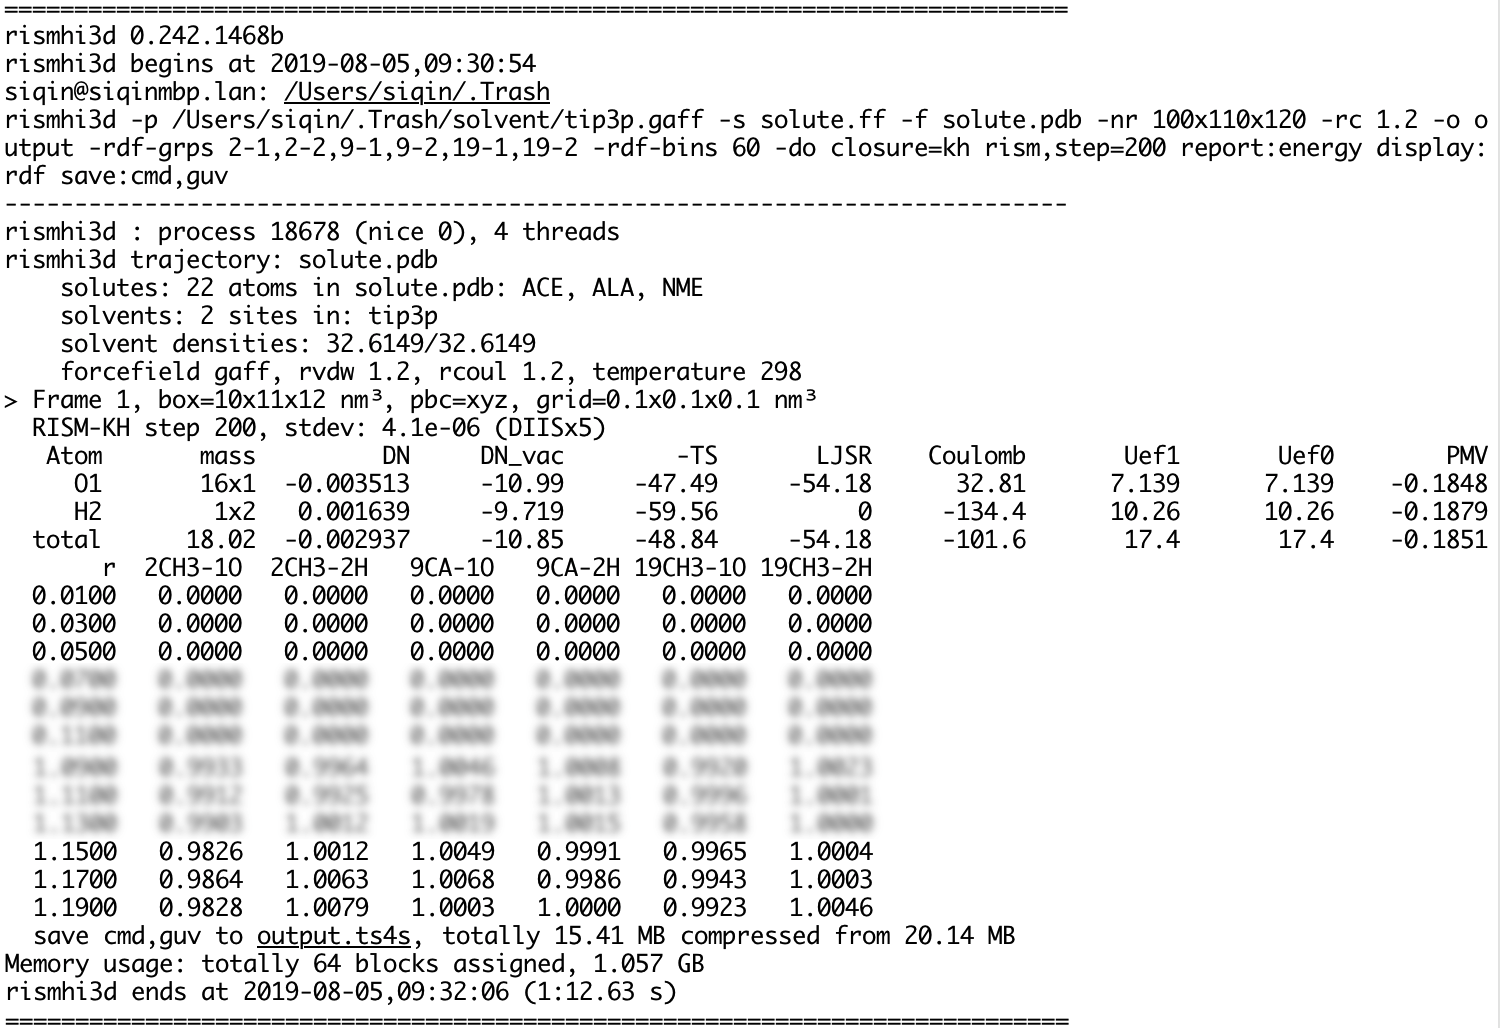
\includegraphics[width=0.7\linewidth]{rismhi3d-demo-screen.png}
	\caption{The screen output of running 3DRISMHI on alanine dipeptide}
	\label{fig:demo-screen}
\end{figure}

The screen output can be seen in Fig. \ref{fig:demo-screen}. At the same time, a file \texttt{output.ts4s} containing the command, density distributions and the HI density distributions is generated in the current folder. This file can be decoded with \texttt{ts4sdump}:

\texttt{\color{blue}\small ts4sdump output.ts4s}

\texttt{\color{blue}\small ts4sdump -e 2 output.ts4s}

\texttt{\color{blue}\small ts4sdump -d 2 output.ts4s}

For hydrophilic solutes, the only RISM need to be performed. For the above example, the 3DRISM-KH calculation can be performed with the following command:

\texttt{\color{blue}\small rismhi3d -p \$IETLIB/tip3p.gaff -s solute.ff -f solute.pdb -nr 60x60x60 -rc 1.2 -do-rism-kh -o output -rdf-grps 6-1,6-2,1-1,2-1 -rdf-bins 60 -log log.txt}

{Again, for advanced users: this command is equivalent to the following command:

\texttt{\color{blue}\small rismhi3d -p \$IETLIB/tip3p.gaff -s solute.ff -f solute.pdb -nr 60x60x60 -rc 1.2 -cmd closure=kh rism report:energy display:rdf savee:cmd,guv -o output -rdf-grps 6-1,6-2,1-1,2-1 -rdf-bins 60 -log log.txt}
}

%\noindent\makebox[\linewidth]{\rule{\linewidth}{0.4pt}}

\section{Input and output}

3DRISMHI work with three input files and some options. The three input files are:
\begin{itemize}
  \item Solvent settings (-p, -solvent, see Sec. \ref{sec:io.solvent}): the information of te solvent
  \item Solute forcefield (-s, -solute, see Sec. \ref{sec:io.solute}): forcefield parameters of the solute
  \item Solute conformation(s) (-f, -traj, see Sec. \ref{sec:io.traj}): the atomic structure of solute molecules
  \item Parameters, options and commands (see Sec. \ref{sec:param}): commands to run, number of grids, number of threads, etc.
\end{itemize}

The output of 3DRISMHI consists of screen outputs, TS4S outputs and RDF outputs:
\begin{itemize}
  \item Screen outputs (see Sec. \ref{sec:io.screen}): brief reports and debug information
  \item TS4S files (see Sec. \ref{sec:io.ts4s}): results in the grid space
  \item RDF file (see Sec. \ref{sec:io.rdf}): text file containing the user-defined RDF pairs
\end{itemize}
By default, only a few screen output will be generated. More details of screen output, TS4S or RDF output will be shown by enabling options or commands (see Sec. \ref{sec:param})

\subsection{Input: Solvent setting file}\label{sec:io.solvent}

The solvent setting file is specified with -p or -solvent. If the current folder doesn't have the solvent setting file, the program will search for the path defined in \$IETLIB. Normally the filename should not begin with ``-'', and if you do have such a file, use ``\texttt{--}'' before the filename (e.g. \texttt{-p -- -solvent\_settings.gaff})

The solvent setting file contains several sections: [solvent], [atom], [bond], and [gvv\_map] ([gvv\_map] is optional).

The {\bf [solvent]} section mainly contains the following parameters:
\begin{itemize}
  \item {\textbf{ff}}: the forcefield type specifier, can be: gaff/amber/opls. The mixing rule of VdW radiuses are arithmetic (-arith-sigma) in gaff/amber or geometric (-geo-sigma) in opls. The energy unit is kJ/mol (-Tdef 120.27) in gaff/opls or kcal/mol (-Tdef 502.97) in amber.
  \item {\textbf{rvdw, rcoul, rc}}: the cutoff distance (in nm) for the interactions. -rc will specify the cutoff for both -rcoul and -rvdw. The LJ interaction is calculated at a hard cutoff at -rvdw, while the Coulomb interaction can be calculated with either a PME swithed at -rcoul (if PME is enabled with -pme) or a hard cutoff at -rcoul (if PME is disabled by -nopme)
  \item {\textbf{density}} and {\textbf{bulk-density}}: a list of the densities or bulk densities of all solvent components. The unit is nm$^{-3}$. The bulk densities are the pure liquid densities of each solvent component.
  \item {\textbf{gvv}}: the solvent-solvent correlations. {\textbf{gvv}} is followed by the name of gvv file and the grid size, e.g. ``-gvv 0.001 tip3p.gvv'' or ``-gvv tip3p.gvv 0.001'' means that the gvv is defined in tip3p.gvv with the grid size of 0.001 nm. The gvv file contains a number of columns, each column is the correlation function of certain pair of solvent sites. The mapping between columns and solvent site pairs are defined by [gvv\_map] section or in a default order (if [gvv\_map] section is missing). The real mapping of gvv can be seen when running the program with ``-list'' option.
  \item {\textbf{zeta}}: the solvent-solvent zeta correlations, only used in HI calculations. The definition of zeta is similar to gvv, while the only difference is the unit of zeta is energy. zeta has no mapping between columns and molecule pairs, and should contain N$\times$N columns for N solvent molecules.
  \item {\textbf{dielect}} or {\textbf{dipole}}: a list of dielectric constants (vacuum is 1) or dipole moments (unit is $\rm e\cdot nm$) of all molecules. The dielectric constants and dipole moments are optional and only used in certain algorithms (e.g. -Coulomb dielect, see Sec. \ref{sec:param} for details)
\end{itemize}

The {\bf [atom]} section defines all the atoms. The [atom] section consists seven columns (more columns are ignored), separated by spaces or tabs:

\begin{center}\begin{tabular}{|c|l|}
    \hline
    column & definition \\
    \hline
    1 & atom name \\
    2 & moleucle name\\
    3 & index \\
    4 & group index \\
    5 & charge \\
    6 & sigma (nm) \\
    7 & epsilon \\
    \hline
\end{tabular}\end{center}

The group index is the site index, and the atoms with the same group (or site) index can be treated as one site in RISM calculation. It is highly suggested that completely equivalent atoms are grouped into one site, which will greatly reduce the computational cost.

The {\bf [bond]} section defines the bonds and pairs of each pair of atoms. The {\bf [bond]} section consists of three or four columes, where the first two columns are the two atoms, and the third column is the bond length or fixed pair distance between the pair of atoms (unit: nm). The fourth column is the RMSD of the fluctuations of bond lengths (or pair distances), which is optional and will be treated as $0$ if the fourth column is missing. Warning: don't define one bond/pair twice.


\subsection{Input: Solute forcefield}\label{sec:io.solute}

The solute forcefield file is specified with -s or -solute. This file contains only {\bf [solute]} section(s). The {\bf [solute]} section contains six or eight (more column are ignored) columns:

\begin{center}\begin{tabular}{|c|c|c|}
    \hline
    column & 6-col format & 8-col format \\
    \hline
    1 & atom name & atom index \\
    2 & moleucle name & atom name \\
    3 & atom mass & residue id \\
    4 & partial charge & moleucle name \\
    5 & sigma (nm) & atom mass \\
    6 & epsilon & partial charge \\
    7 & & sigma (nm) \\
    8 & & epsilon \\
    \hline
\end{tabular}\end{center}

The solute forcefield can be simply translated from the GROMACS top file with the ``gmxtop2solute'' tool provided in the software package.


\subsection{Input: Solute conformation(s)}\label{sec:io.traj}

The solute conformation(s) are defined in the trajectory file, specified with -f or -traj. The trajectory file can be a PDB, GRO or XTC file.

The PDB file: only lines begin with ``ATOM'' or ``CRYST1'' will be processed. The number of atoms defined by the ATOM lines should be consistent with the solute forcefield file. The box size should be defined with a CRYST1 line. The PDB file can contain multiple frames, separated by ``ENDMDL''.

The GRO file can also contain multiple frames.

The XTC file can be processed only when the software is compiled with \_GROMACS\_ options. It's fine to turn off all \_GROMACS\_ flags when compling the software, as long as you don't have GROMACS or don't want to be bothered by this feature. The frames of XTC between the time (in ps) defined in {\bf -b} and {\bf -e} are handled, and {\bf -dt} specifies the time interval between frames that handled in 3DRISMHI.


\subsection{Output: screen report}\label{sec:io.screen}

The screen output consists of the information of running and some brief reports of calculation results.

The running information can be muted with {\bf -v 0}. If you want to monitor the status of running, please use {\bf -v 1}, {\bf -v 2} or simply {\bf -v}.

More running information is shown in debug mode. {\bf -debug 0} will mute all debug message, and {\bf -debug 1} will allow to show some important messages (e.g. real location of input files, allocated memory, thread, etc.). In {\bf -debug 2}, a detailed running process is printed on screen, including calling of major functions in the source code. Further in {\bf -debug 3} or {\bf -debug-crc}, the CRC check sum of important memory bulks will be displayed on the screen. Please note that -debug 3 or -debug-crc will perform the CRC calculation, which will require additional computing time.

A detail report of time consumption will be displayed at the end with {\bf -v 2} or {\bf -debug 1/2/3}.

The brief reports of calculation results will be displayed according to the command defined in the command queue. Please see Sec. \ref{sec:param} for details of commands and the command queue. For example, if you want a detailed report of energy or correlation functions, you need to add a ``-cmd report:energy'' or ``-cmd report:cuv'' command; if you want to show the rdf, you need to add a ``-cmd display:rdf'' command.

The screen output can be redirected to a log file specified with {\bf -log} ({\bf -log screen}, {\bf -log stdout} and {\bf -log stderr} will redirect the screen output to stdout or stderr).

\subsection{Output: TS4S file}\label{sec:io.ts4s}

The TS4S file contains one or more frames of 4D tensors. Normally in 3DRISMHI, the 4D tensors can be LJ potentials, Coulomb potentials, total correlation, direct correlation, total density profile and HI density.

The name of the output TS4S file is specified with {\bf -o[v][0/1/2]} or {\bf -a[0/1/2]}, where ``ov'' represepts overriding, and ``a'' represents appending. The TS4S data can be uncompressed ({\bf -o[v]0} or {\bf -a0}) or compressed with ZLIB (if you compiled with the \_ZLIB\_ option). Please note that the TS4S file may be extrodinarily huge, and the {\bf -significant-digits} or {\bf -sd} option may be helpful for higher compressibility with lower accuracy of output data (e.g. {\bf -sd 5} will keep only five significant digits, and {\bf -sd float} will trim all output data to float).

The output of TS4S will be performed with the ``save'' command defined in the command queue (see Sec. \ref{sec:param} for details). The TS4S file will be generated at the first saving command. The filename extension of TS4S is always ``.ts4s''. If the filename is not specified, a default filename solute.solvent.YYMMDD\_HHMM.ts4s will be used.

Please use ``ts4sdump'' (provided in the software package) to check and decode the TS4S file.

{\it (For developer:) The file format of a TS4S file is defined in compress.cpp of the source code. TS4S consists a number of data blocks, each block corresponding to a 4D tensor. One 4D tensor block begins with the IETSPageHeader structure, followed by comment text and tensor data. The decoded 4D tensors are organized in the order of ``tensor[solvent\_site][z][y][x]''.}

\subsection{Output: RDF file}\label{sec:io.rdf}

The RDF can be calculated and displayed or written to a text file. The RDF groups are defined in ``{\bf -rdf-grps} u1-v1,u1-v2,...'', where u1, u2 ... stand for the indexes of solute atoms and v1, v2 ... stand for the indexes of solvent sites. The number of RDF bins is defined in ``{\bf -rdf-bins} 50'', where 50 is the default bin number. The RDF will be performed up to the distance defined in ``{\bf -rc}''. For an advanced user who wants to see the RDFs of HI densities or direct correlations, the ``{\bf -rdf-content}'' option can be used to specify the RDF to calculate: rdf (density profile, by default), h (direct correlation), dd (HI density), c (direct correlation), ch (ch=$c*h$), lj (LJ potential) or coul (Coulomb potential).

The displaying or saving of RDF is performed in ``-cmd display:rdf'' or ``-cmd save:rdf''. The RDF is calculated when necessary, so no RDF calculation will be performed if the RDF is not displayed or saved. ``-cmd display:rdf'' will display the RDF on screen (or -log file), while ``-cmd save:rdf'' will save the RDF to a text file. The name of the RDF file begins with the name of TS4S file, and ended with a ``.rdf'' extension.


%\noindent\makebox[\linewidth]{\rule{\linewidth}{0.4pt}}

\section{Parameters, options and commands}\label{sec:param}

\subsection{Parameters for running}\label{sec:param.param}

In the command line parameters, you can specify the running parameters, tell the software what to compute and display, and override some solvent settings. (Please note that all the settings in the {\bf [solvent]} section can be overridden by the command line parameters.) Here is a list of the major parameters for running:

\begin{itemize}
    \item {\bf -nt} and {\bf -np}: number of parallel runnings. -np 1 or -nt 1 will disable the paralleling. {\bf -nt} will use pthread while {\bf -np} will use fork. Please note that paralleling is still possible (with -np) even if you hate or don't have pthread. {\bf -np} is enabled with \_LOCALPARALLEL\_ option in compiling, while {\bf -nt} requires both \_LOCALPARALLEL\_ and \_LOCALPARALLEL\_PTHREAD\_ in compiling. Note: the 3DRISMHI will automatically set -nt to the maximum number of your CPU cores. So don't forget to change -nt or -np if you are running 3DRISMHI on a cluster.

        An important thing of paralleling is that the \_LOCALPARALLEL\_FFTW\_ will manually parallelize the FFTW by performing multiple FFTWs at the same time. For an N site (or molecule) system, N$\times$N FFTWs need to be performed in one RISM (or HI) iteration, thus the maximum number of working threads in \_LOCALPARALLEL\_FFTW\_ mode is N$\times$N (more threads will be idling). For example, if your solvent contains nothing but water (one molecule and two sites), then only one thread/process will be busy in the HI convolutions and at most four threads/processes will be busy in the RISM convolutions.

        Other parts of massive computations (i.e. building forcefield and performing DIIS) will make full use of multi threads/processes.
    \item {\bf -ntf}: number of threads for FFTW. This is enabled with multithread FFTW. This opention does little or negligible improvement of the computation efficiency.
    \item {\bf -nice}: the nice level of running this software.
    \item {\bf -nr }: the grid number. It can be one number for both three dimensions; three numbers for X, Y and Z respectively; or NXxNYxNZ. e.g. ``-nr 50'' is equivalent to ``-nr 50 50 50'' and ``-nr 50x50x50''. The grids of X, Y and Z can be different, e.g. ``-nr 50x60x70''. The grid numbers are suggested to be even numbers.
    \item {\bf -step} 100: set the maximum steps for HI and RISM.
    \item {\bf -interact}: enable the interactive mode. Pressing enter at running will halt the calculation, and you can print the report, change parameters, continue running, end current RISM/HI calculation or quite the program. Warning: don't enable the interactive mode when you are running 3DRISMHI in background (e.g. nohup or on a cluster).
    \item {\bf -do-rism-kh}, {\bf -do-rismhi-kh} and {\bf -do-rismhi-d2}: perform 3DRISM or 3DRISMHI with the KH or D2MSA closures. The RDFs will be displayed on screen if {\bf -rdf-grps} are defined, while a TS4S file containing the running command and the density distributions will be generated if the output file is specified.
    \item {\bf -cmd} or {\bf -do}: the command(s) you want to run. The software will do nothing if the command queue is empty. See Sec. \ref{sec:param.command} for details.
    \item {\bf -skip-missing-xvv} never or {\bf -skip-zero-xvv} never: skip the convolution related to fully zero solvent-solvent correlations (including wvv, nhkvv and zeta). This option is disabled by default, and can be enabled by {\bf -skip-missing-xvv} [yes] or {\bf -skip-zero-xvv} [yes]. This option should yield exactly the same results (including the CRC checksum) as not enabled while significantly faster as fewer FFT is required to be performed.
\end{itemize}

And here is a list of some important {\bf [solvent]} settings that can be redefined:

\begin{itemize}
    \item {\bf -temperature} 298: specify the temperature in Kelvin
    \item {\bf -Tdef} 120.27: specify the temperature of defining the energy unit. 1 kJ/mol = 120.27 K, 1 kcal/mol = 502.97 K. Can be specified with {\bf -ff}.
    \item {\bf -arith-sigma} and {\bf -geo-sigma}: set the combing rule of VdW raiuds to arithmetic or geometric averaging.
    \item {\bf -density} and {\bf -bulk-density} can be redefined in the command line parameters.
    \item {\bf -ndiis}, {\bf -ndiisrism} and {\bf -ndiishi}: the maximum steps of DIIS. More steps of DIIS will have better convergence of self-consistent-field iterations while require more memory.
    \item {\bf -delvv}, {\bf -delrism} and {\bf -delhi}: the step in factor of the self-consistent-field iterations. {\bf -delvv} for both RISM and HI. Both are 1 by default, and 0.7 is recommended by RISM.
    \item {\bf -errtol}, {\bf -errtolrism} and {\bf -errtolhi}: the error tolerance of convergence. Both are $10^{-12}$ by default. Although this is fine for HI, the RISM iterations have little chances to reach the error of $10^{-12}$. This number is suggested to be $10^{-7}$ in AMBER RISM.
    \item {\bf -bound-to-ram} or {\bf -ignore-memory-capacity}: by default, the software will detect the capacity of the physical memory, and will terminate when the memory is exceeding the physical memory. This feature can be disabled by {\bf -ignore-memory-capacity}, which will cause extremely low computational efficiency as well as high risk to damage your hard disk. Ignore the memory capacity check only when you know what you are doing.
\end{itemize}

Other advanced options can be seen in Sec. \ref{sec:param.options}

\subsection{Commands and command queue}\label{sec:param.command}

The command forms a command queue, and will be performed one by one after the frames are read from the trajectory file. The command(s) specified in {\bf -cmd} will be added to the command queue. You can use \@ to relocate the current command instead of inserting it to the end of the queue, e.g. ``-cmd report@5:energy'' will insert ``-cmd report:energy'' to the 5th command (the command queue begins with 1). \@b and \@e can be used to force the command to runs before handling of any frame or after handling all frames, e.g. ``-cmd report:rdf'' will report the RDF at each frame, and ``-cmd report@end:rdf'' will report the overall RDF after all frames have been processed.

Followings are some basic commands for setting closures, running HI/RISM calculations, and generating reports or output files of the output results:

\begin{itemize}
    \item {\bf build-ff}: {\bf -cmd build-ff}: force to rebuild the forcefield. The forcefield is built automatically with {\bf rism} or {\bf hshi}, and this command is used only when you need to do something without perfoming RISM or HI.

    \item {\bf rism}: {\bf -cmd rism},step=100: perform 3DRISM with specified number of maximum steps and the closure(s) defined in the {\bf closure} command before.
    \item {\bf ssoz}: {\bf -cmd ssoz},step=100: perform unrenormalized 3DRISM with specified number of maximum steps and the closure(s) defined in the {\bf closure} command before. The unrenormalized 3DRISM is the very original version of 3DRISM, which has big issues in electrostatic interactions.
    \item {\bf hshi}: {\bf -cmd hshi},step=100: perform HI with specified number of maximum steps.

    \item {\bf closure}: {\bf -cmd closure=}closure\_A[,closure\_B,...]: set the closure(s) for each molecule. Different sites can be calculated with different closures, and at most 20 closures are allowed to be specified here. Particularly, all the sovlent sites will use the same specified closure if only one closure is given here. This version of 3DRISMHI support all the closures mentioned in Sec. \ref{sec:closure}: HNC, MSA, KGK, PLHNC, KH, PSE2, PSE3, ... PSE10, PY, HNCB, D2, MS, MSHNC, BPGGHNC, VM, MP.
    \item {\bf closure-a}: set the closure(s) for each site instead of molecule.
    \item {\bf closure-factor}: {\bf -cmd cf=}cf\_A[,cf\_B,...]: set the extra parameters that used in closures.

    \item {\bf report}: {\bf -cmd report:}Euv/energy/cuv/rdf: generate a report on screen (or to -log file). {\bf -cmd report:Euv} will display a brief report of total energies, while {\bf -cmd report:energy} will display a detailed report of total energies. {\bf -cmd report:cuv} will display the total direct correlations, and {\bf -cmd report:rdf} will display the RDFs if you have defined the RDF groups. In addition, {\bf -cmd report:energy,cuv} is equivalent to {\bf -cmd report:all}.
    \item {\bf display}: {\bf -cmd display:}lj/coul/Euv/energy/cuv/dN/dN0/TS/GGF/rdf: display the values of the chosen variables
    \item {\bf save}: {\bf -cmd save:}cmd/lj/coul/cuv/huv/hlr/dd/ddp/nphi/guv/rmin/rdf: save the specified quantity. {\bf -cmd save:cmd} will save the command line arguments to the TS4S file, and {\bf -cmd save:guv} will save the density distributions of each solvent site at each spacial grid to the TS4S file. {\bf -cmd save:lj,coul,cuv,huv,hlr,dd} will save LJ potentials, Coulomb potentials, direct correlations, total correlations, long range total correltations, HI density to the TS4S file, and {\bf -cmd save:rmin} will save the minimal-to-solute distances to the TS4S file. Additionally, {\bf -cmd save:rdf} will save the RDF to the RDF file (which is a text file).
    \item {\bf savee}: mostly the save as {\bf save}. The only difference is that {\bf savee} will perform saving only when the output TS4S file is explicitly specified, while {\bf save} will use an default filename if the output TS4S file is not explicitly specified.
\end{itemize}

Addtionally, some shortcuts can be used to add a bundle of commands. Don't use two or more shortcuts, otherwise both the two sets of commands will be performed.

\begin{itemize}
    \item {\bf -do-rism-kh} = -cmd closure=kh rism report:energy display:rdf savee:cmd,guv
    \item {\bf -do-rismhi-d2} = -cmd hshi closure=d2 rism report:energy display:rdf savee:cmd,guv
    \item {\bf -do-rismhi-kh} = -cmd hshi closure=kh rism report:energy display:rdf savee:cmd,guv
\end{itemize}

\subsection{Other options}\label{sec:param.options}

Below is a list of major advanced options that can be defined in both the {\bf[solvent]} section of the solvent setting file or the command line parameters:

\begin{itemize}
    \item {\bf -lsa} and {\bf -lsb} for HI: the two parameters, $A$ and $B$ of the liquid equation of state \cite{Cao_Xuhu_JCP_2015, Cao_Xuhu_MP_2018, Cao_Huang_AdTS_2019}. $B$ is automatically computed, and $A$ can be defined with {\bf -lse-a} or {\bf -lsa}. The recommended values of $A$ can be seen from previous experimental measurements \cite{DYMOND_IJT_1988}.
    \item {\bf -theta} for HI: define the energy cutoff (in kT), above which the regions are treated as hard cores or no solvent regions. The default cutoff is 5 kT.
    \item {\bf -Coulomb}: the preprocessing algorithm of the Coulomb interactions in HI and RISM. Can be: none (=-Coulomb), dielect, or Yukawa.
    \item {\bf -Yukawa} 0.5: the same as {\bf -Coulomb Yukawa} 0.5. 0.5 here is the characteristic length (unit: nm) of the exponential function of the Yukawa potential. The Debye length of homogeneous bulk liquid will be used if the characteristic length is not specified. The dielectric constant for the Yukawa potential is defined in {\bf -dielect-y}.
    \item {\bf -rb} or {\bf -Bohr-radius}: the minimal raiuds of an atom. By default it is 0.052911 (nm).
    \item {\bf -sd} or {\bf -significant-digits}: the significant digits in the TS4S files, can be ``float'', ``double'' or a number (significant digits in decimal)
    \item {\bf -closure-enhance-level} 1 or {\bf -enhance-closure} 1: scale down the changes of SCF iterations with $(1+h^2)^{\alpha/2}$, where $\alpha$ is the closure enhancement level. This option greatly improves the convergence of the self-consistent-field iterations and is turned on by default. Use {\bf -no-closure-enhance} to turn this feature off.
    \item {\bf -bounded-to-ram}: don't exceed the physical memory capacity when using memory. This feature is on by default, and use {\bf -ignore-memory-capacity} to turn this feature off.
    \item {\bf -xvv-extend} 0: extend the {\bf gvv} of solvent. If the input gvv contains the RDFs of $2$ nm, then -xvv-extend 5 will extend it to $10$ nm by filling the extended regions with $1$. This option is helpful when you {\bf gvv} is poor, but don't expect too much.
\end{itemize}


\bibliography{user-manual}

%\input{experimental-features.tex}

\end{document}
